\documentclass[11pt]{article}
\setlength{\textheight}{240mm}
%\setlength{\voffset}{0mm}
\addtolength{\topmargin}{-30mm}
\setlength{\textwidth}{155mm}
\setlength{\oddsidemargin}{5mm}
\usepackage{graphicx, caption, subcaption}
\graphicspath{ {./figs/} }
\pagestyle{plain}
\begin{document}
\title{Edge Reconnecting Coarse Projective Integration}
\author{Alexander Holiday\vspace{-2ex}}
\date{09/10/2013}
\maketitle
\section*{Introduction}
The edge reconnecting model, detailed in \cite{balazs:rsa12}, was implemented in C++. The system naturally converges to a limiting ``graphon'' (see \cite{lovasz:jcombth06}), and in order to increase the rate of convergence, coarse projective integration (CPI) was implemented. This brief outlines the model dynamics and reviews current simulation progress.

\section*{Edge Reconnecting Model}
The initial state of the edge reconnecting model is an Erd\H{o}s-R\'{e}nyi random graph with $n$ vertices and $m\sim O(n^{2})$ edges. The system evolves as a discrete-time Markov chain, in which the following actions are performed during each step:

\begin{enumerate}
\item An edge, $e_{old}$, is chosen uniformly at random from the set of all possible edges, $E(G)$.
\item A vertex end of $e_{old}$, $v_{1}$, is chosen uniformly from the two ends.
\item $e_{old}$ is removed from the graph, and a vertex $v_{2}$ is chosen from $V(G)$ with a probability based on linear preferential attachment:
  \[
  P(v_{2}=v_{i})=\frac{deg(v_{i})+\kappa}{2m+n\kappa}
  \]
where $\kappa$ is a model parameter and $deg(v_{i})$ denotes the degree of vertex $i$ in $V(G)$.
\item An edge, $e_{new}$, is added between $v_{1}$ and $v_{2}$.
\end{enumerate}

Two distinct timescales arise from these dynamics, $T\asymp n^{2}$ and $T\asymp n^{3}$ where $T$ is the number of steps. On the faster, $O(n^{2})$ scale, the degrees of the vertices may be considered constant, while the number of parallel edges between vertices changes. On the slower $O(n^{3})$ scale, the degree distribution evolves to a steady state value. While this separation of timescales has been proven in \cite{balazs:rsa12}, identifying them through numerical simulations is complicated by a couple of factors. First, the exact timescales themselves are difficult to discern. Both scales are really $O(\rho_{1} n^{2})$ and $O(\rho_{2} n^{3})$, where the constants $\rho_{i}$ are evaluated at the limit of infinite-sized graphs ($n\rightarrow \infty$). This hints at the second, larger, problem: many of the results on the existence of these timescales in the first place are only valid in this large-$n$ limit. Simulation time then becomes problematic. Figs. \ref{fig:degSurf100} and \ref{fig:degSurf500} illustrate attempts to visualize these separate scales of evolution. The degree distribution is plotted every $n^{2}$ steps in thse figures, with a total number of $n^{3}$ steps in each. The changes appear quite gradual, and no distinct timescales are evident.\\
\indent In spite of the difficulties in accurately locating these different regions, progress has been made towards performing CPI on the system. Current work to this end is outlined below.
\clearpage

\begin{figure}[h]
  \begin{minipage}[c][11cm][t]{.9\textwidth}
    \centering
    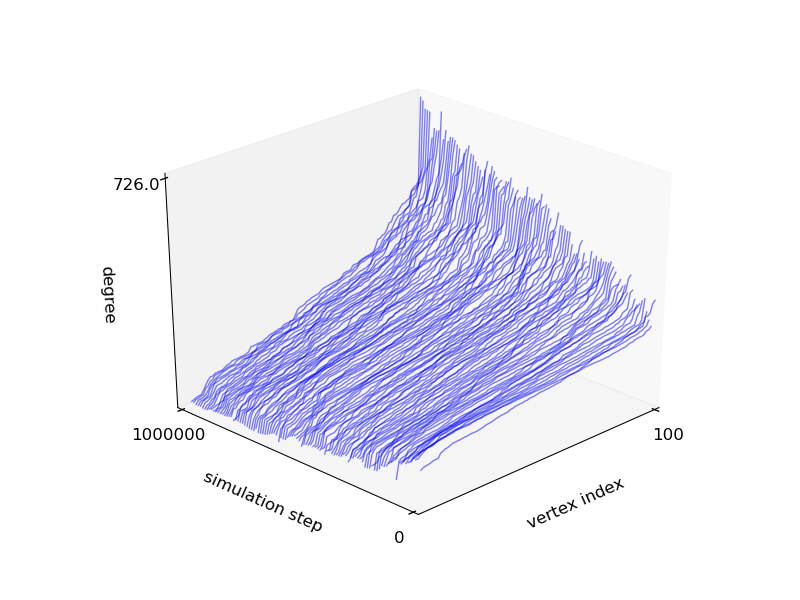
\includegraphics[width=127mm]{degSurf100}
    \subcaption{$n=100$}
    \label{fig:degSurf100}\par\vfill
  \end{minipage}
  \begin{minipage}[c][11cm][t]{.9\textwidth}
    \centering
    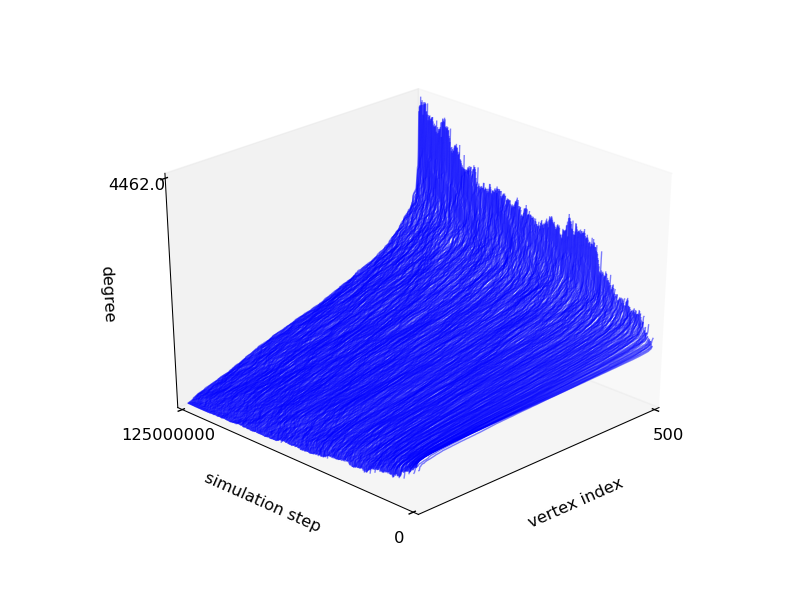
\includegraphics[width=127mm]{degSurf500}
    \subcaption{$n=500$}
    \label{fig:degSurf500}
  \end{minipage}
  \caption{Evolution of degree distribution for $n^{3}$ steps}
\end{figure}
\vspace{10cm}

\clearpage
\section*{CPI}
Our approach in coarse-graining system dynamics is based on the existence of a gap in the spectrum of the adjacency matrix, and the subsequent ability to approximate $A\approx \lambda_{1}v^{(1)}v^{(1) \;\dagger}$ where $A$ is the adjacency matrix of the system, $\lambda_{1}$ is the leading eigenvalue of $A$, and $v^{(1)}$ the corresponding eigenvector. Fig. \ref{fig:spectralGap} shows that clearly $|\lambda_{1}| \gg |\lambda_{i}|, i=2,3,...,n$. 

\begin{figure}[h]
  \centering
  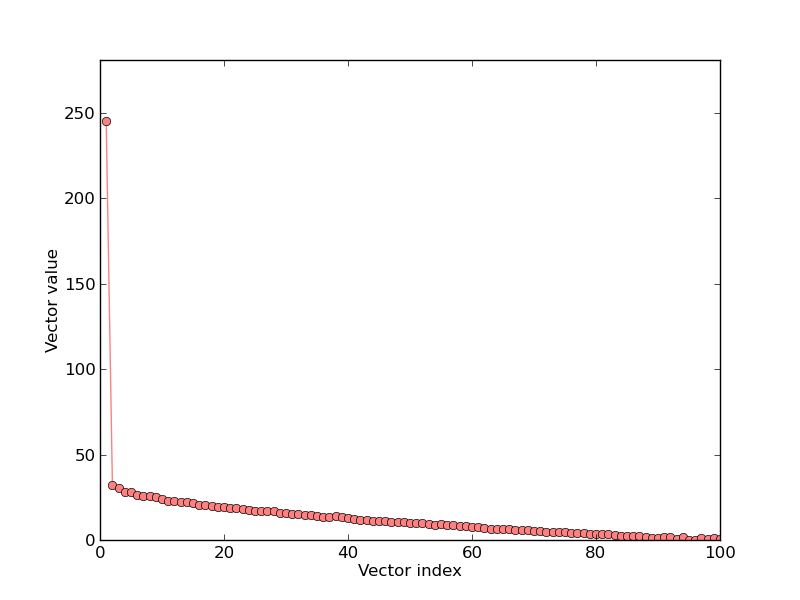
\includegraphics[height=10cm]{spectralGap100}
  \caption{Eigenvalues of $A$, $n=100$}
  \label{fig:spectralGap}
\end{figure}

Fig. \ref{fig:adjRecon} illustrates the reconstruction of the adjacency matrix as $A_{i,j}=\lambda_{1}v^{(1)}_{i,j}v^{(1) \;\dagger}_{i,j}$ (after multiplication, each entry $A_{i,j}$ was rounded to the nearest integer if $i\neq j$ or to the nearest even integer if $i=j$). Visually, the two correspond very well.

\begin{figure}[h!]
  \begin{minipage}[c][10cm][t]{.9\textwidth}
    \centering
    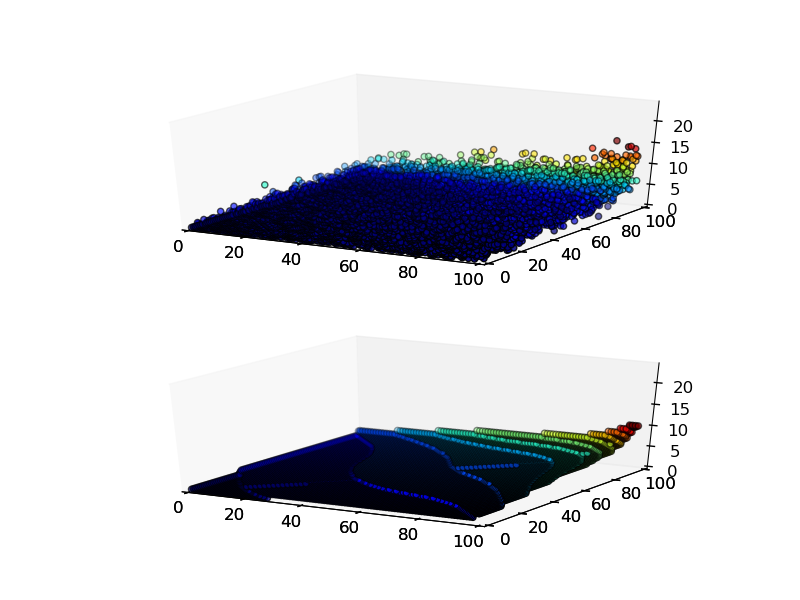
\includegraphics[width=12cm]{adjReconShort100}
    \subcaption{Early in simulation run (maximum degree remains small)}
  \end{minipage}
  \begin{minipage}[c][10cm][t]{.9\textwidth}
    \centering
    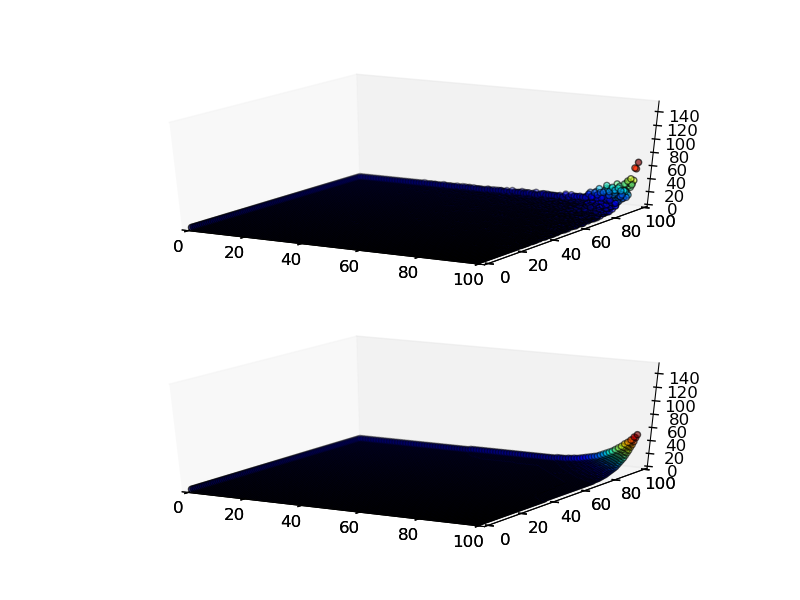
\includegraphics[width=12cm]{adjReconLong100}
    \subcaption{\centering Further into simulation (preferential attachment causes a few vertices to attain very large degrees)}
  \end{minipage}
  \caption{Original adjacency matrices taken from simulations (top of each subfigure) and their reconstruction from the leading eigenvalue/eigenvector pair (bottom), $n=100$. Please note: the color adds no information to the plots: it scales directly with the z-axis and can (probably should) be taken out of the image}
  \label{fig:adjRecon}
\end{figure}
 
\clearpage

\begin{figure}[h]
  \centering
  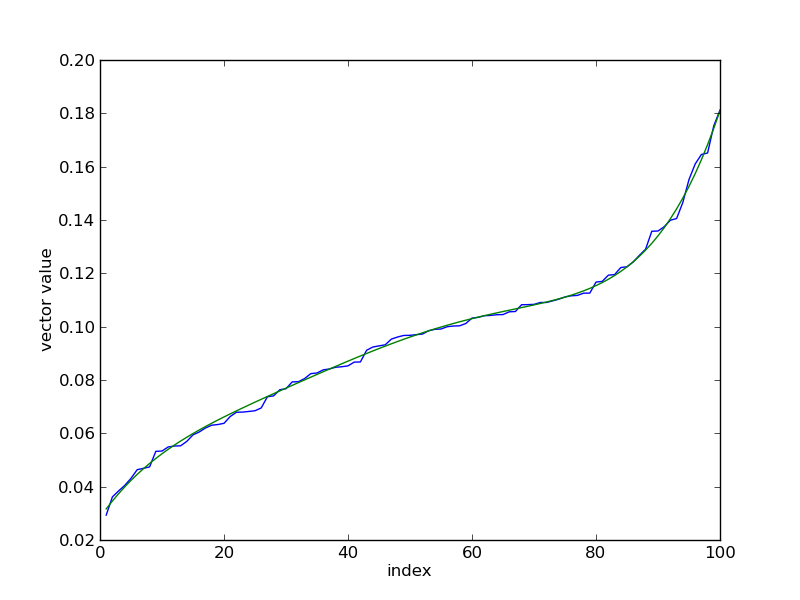
\includegraphics[height=10cm]{eigVectFitting}
  \caption{Eigenvector from simulation (blue), and its approximation by a fifth-order polynomial (green)}
  \label{fig:eigVectFitting}
\end{figure}
As $\lambda_{1}v^{(1)}v^{(1) \;\dagger}$ appears a good approximation of $A$, it was reasoned that we could use this eigenvalue/eigenvector combination as a coarse description of $A$. In order to further reduce dimensionality, the eigenvector was fitted with a fifth-degree polynomial, as shown in Fig. \ref{fig:eigVectFitting}. The six coefficients of this function were then used as a smaller set of coarse variables, leading to a final seven-dimensional representation of the system (six coefficients plus an eigenvalue). The following outlines the CPI framework:

\begin{enumerate}
\item Simulate the full edge reconnecting model dynamics for some number of steps until the fast variables are sufficiently slaved to the slow
\item Record the adjacency matrix as the system evolves on the slow manifold (in fact, it is more efficient to immediately compute the leading eigenvector, fit it with a polynomial, and store only these coefficients, along with the leading eigenvalue, as time progresses)
\item Project forward the coarse variables (coefficients and eigenvalue)
\item Reconstruct a new adjacency matrix from the new, projected coefficients and eigenvalue:
  \begin{enumerate}
  \item Compute a new eigenvector as $v(i) = \displaystyle\sum\limits_{k=0}^{k=6} i^{k}c_{k}$ (where $c_{k}$ represents the coefficients of the polynomial and $v(i)$ the $i^{th}$ component of $v$) and round to the nearest integer
  \item Compute the new adjacency matrix as $A_{i,j}=\lambda_{1}v^{(1)}_{i,j}v^{(1) \;\dagger}_{i,j}$ and round as discussed previously
  \end{enumerate}
\item Repeat step one until system reaches steady state
\end{enumerate}

Preliminary results of this method are shown in Fig. \ref{fig:CPI}, in which the evolution of the degree distribution is shown for both the full simulation and a simulation in which CPI has been employed.

\begin{figure}[h]
  \centering
  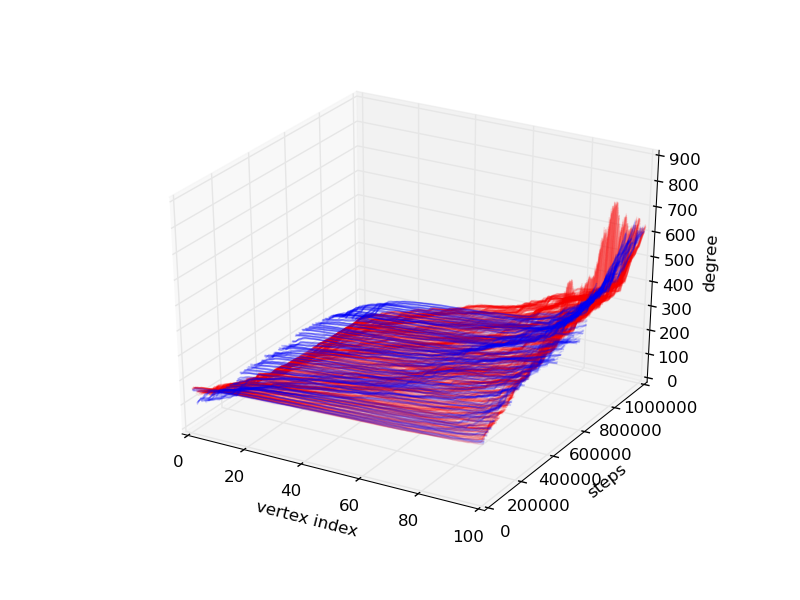
\includegraphics[height=10cm]{CPI}
  \caption{Overlay of degree distribution evolution for full simulation (red) and projective integration (blue)}
  \label{fig:CPI}
\end{figure}

\section*{Future work}
The largest obstacle to further progress is the accurate identification (through simulation) of the disparate timescales present in this system's dynamics. Once these are found, a more efficient and accurate CPI method should readily follow.

\bibliographystyle{abbrv}
\bibliography{/home/oakridge/holiday/Documents/latex/bib}
\end{document}
